% The 10×5 grid of digits with the column sums underneath — Numbers 30 of the
% abacus (Hard). Transcribed from the original scan; the givens are the puzzle,
% so they must match it cell for cell.
%
% Wordless (digits read the same in both languages), so it builds once. Line art
% only: every stroke is black and gets rewritten to currentColor, which is also
% why the sums strip is left unfilled — a light band would swallow the white
% strokes on the dark theme.
\documentclass[tikz,dvisvgm,border=3pt]{standalone}
\begin{document}
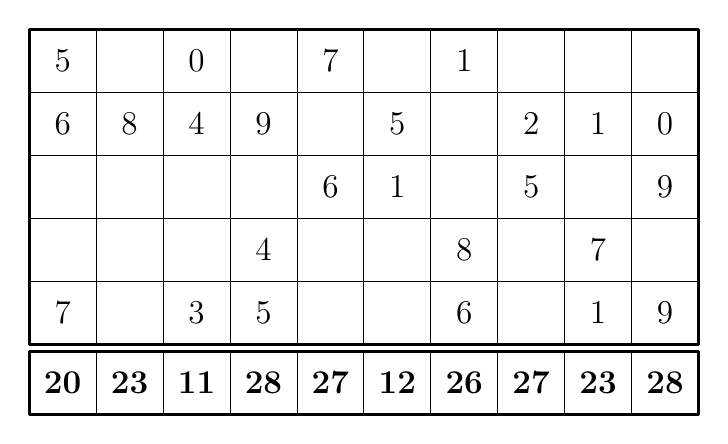
\begin{tikzpicture}[
  x=0.85cm, y=0.8cm,
  line join=round,
  cell/.style={line width=0.3pt},
  frame/.style={line width=1.1pt},
  num/.style={font=\large},
  sum/.style={font=\large\bfseries},
]

% ── the givens ────────────────────────────────────────────────────────────
\foreach \c/\r/\v in {%
  1/1/5, 3/1/0, 5/1/7, 7/1/1,
  1/2/6, 2/2/8, 3/2/4, 4/2/9, 6/2/5, 8/2/2, 9/2/1, 10/2/0,
  5/3/6, 6/3/1, 8/3/5, 10/3/9,
  4/4/4, 7/4/8, 9/4/7,
  1/5/7, 3/5/3, 4/5/5, 7/5/6, 9/5/1, 10/5/9%
} { \node[num] at (\c-0.5,-\r+0.5) {\v}; }

% ── the grid ──────────────────────────────────────────────────────────────
\foreach \c in {1,...,9} { \draw[cell] (\c,0) -- (\c,-5); }
\foreach \r in {1,...,4} { \draw[cell] (0,-\r) -- (10,-\r); }
\draw[frame] (0,0) rectangle (10,-5);

% ── the column sums, in a strip of their own ──────────────────────────────
\draw[frame] (0,-5.12) rectangle (10,-6.12);
\foreach \c in {1,...,9} { \draw[cell] (\c,-5.12) -- (\c,-6.12); }
\foreach \c/\v in {1/20, 2/23, 3/11, 4/28, 5/27, 6/12, 7/26, 8/27, 9/23, 10/28}
  { \node[sum] at (\c-0.5,-5.62) {\v}; }

\end{tikzpicture}
\end{document}
